\section{Robustness analysis}

After introducing the alterations to be applied to assess the model robustness, we generated altered datasets for each alteration. Specifically, we uniformly sampled 20 points from each alteration range. The subsequent step involves evaluating the networks on these altered datasets to compute the necessary metrics. For the standard NN, only accuracy is computed, whereas for the BNN, additional metrics include the unknown ratio and effectiveness. Moreover, the BNN metrics will be calculated using different classification methods introduced in \Chap~\ref{chap:c3}. The classification method with uncertainty penalization will not be used, as it has proven to be ineffective in this application.

As mentioned at the beginning of this chapter, the definition of robustness used is the one in \Def~\ref{def:rob3}, with linear tolerance, zero threshold, and a $maxAcc$ set to the nominal accuracy. Since $\Theta=0$, there is no penalization function, resulting in a metric ranging from $0.5$ in the worst-case scenario to $1$ in the best-case scenario.

For the BNN, robustness against indecision will also be computed based on \Def~\ref{def:robind}, employing a linear tolerance, $\gamma=100$, and the nominal unknown ratio as the baseline. Additionally, we will calculate augmented robustness following \Def~\ref{def:robaug}, which uses the effectiveness as well.

\subsection{Gaussian noise}

\Fig~\ref{fig:acc_gn_wu} shows the results of obtained using the altered data with gaussian noise. In particular, \Fig~\ref{fig:gn_acc_wu_bnn} shows the accuracy trend of the BNN while \Fig~\ref{fig:gaus_noise_ann} the one for the standard NN. It is possible to see that the behavior is basically the same, although the standard ANN seems to be slightly more robust. The degradation in accuracy shows a linear behavior with respect to the noise variance.

\begin{figure}[h]
	\centering
	\begin{subfigure}{.5\textwidth}
		\centering
		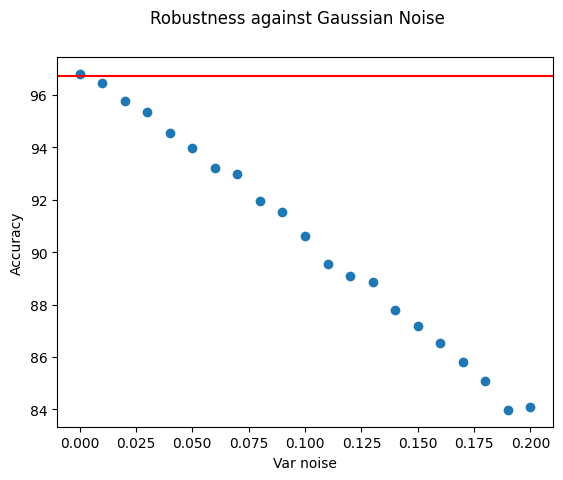
\includegraphics[width=0.9\linewidth]{ImageFiles/EvalBNN/GN/WU/acc}
		\caption{BNN}
		\label{fig:gn_acc_wu_bnn}
	\end{subfigure}%
	\begin{subfigure}{.5\textwidth}
		\centering
		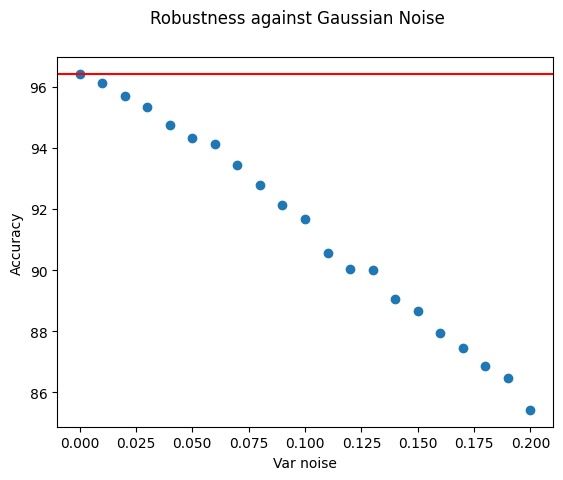
\includegraphics[width=0.9\linewidth]{ImageFiles/EvalANN/gaus_noise_ann}
		\caption{Stanard NN}
		\label{fig:gaus_noise_ann}
	\end{subfigure}
	\caption{Accuracy trend for gaussian noise}
	\label{fig:acc_gn_wu}
\end{figure}

\todo{boh}
Computing the robustness it results in $boh$ for the and $boh$ for the standard NN.  These values are quite close to $1$, indicating that both networks exhibit good robustness to Gaussian noise.

\Fig~\ref{fig:gn_uncertainty}displays the trend of uncertainty estimated by the BNN. Specifically, \Fig~\ref{fig:gn_aleatoric} illustrates the aleatoric uncertainty trend, while \Fig~\ref{fig:gn_epistemic} presents the epistemic uncertainty.

It is worth noting that both uncertainties increase approximately linearly with respect to the noise variance. This shows that input data altered with gaussian noise makes the network less certain about its predictions and the uncertainty linearly proportional to the noise variance.

\begin{figure}[h]
	\centering
	\begin{subfigure}{.5\textwidth}
		\centering
		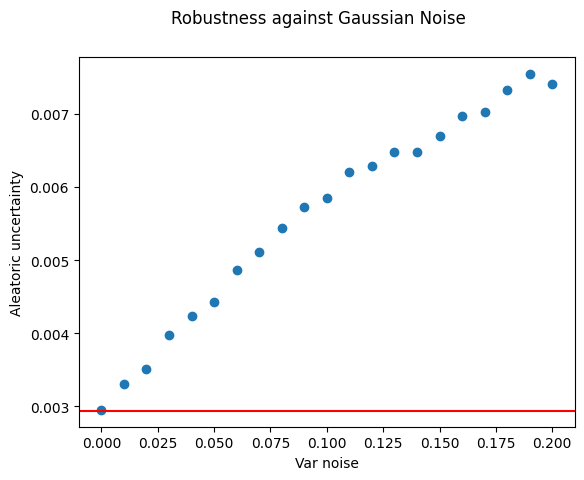
\includegraphics[width=0.9\linewidth]{ImageFiles/EvalBNN/GN/aleatoric}
		\caption{Aleatoric uncertainty}
		\label{fig:gn_aleatoric}
	\end{subfigure}%
	\begin{subfigure}{.5\textwidth}
		\centering
		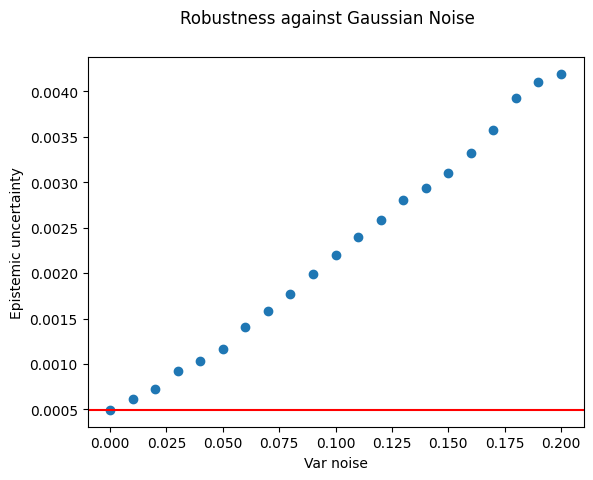
\includegraphics[width=0.9\linewidth]{ImageFiles/EvalBNN/GN/epistemic}
		\caption{Epistemic uncertainty}
		\label{fig:gn_epistemic}
	\end{subfigure}
	\caption{Uncertainty trend for gaussian noise}
	\label{fig:gn_uncertainty}
\end{figure}


The next analysis will focus on evaluating whether the utilization of estimated uncertainty contributes to performance improvement.